
\documentclass[aspectratio=169]{beamer}

% -----------------------------------------------------
% THEME AND PACKAGES
% -----------------------------------------------------
\usetheme{Madrid}
\usecolortheme{seahorse}

\usepackage[T1]{fontenc}
\usepackage{lmodern}
\usepackage{listings}
\usepackage{xcolor}
\usepackage{tikz}
\usepackage{booktabs}
\usepackage{array}
\usepackage{amsmath}

\usetikzlibrary{
    arrows.meta,
    positioning,
    shapes.geometric
}

% -----------------------------------------------------
% COLORS
% -----------------------------------------------------
\definecolor{codebg}{RGB}{248,248,248}
\definecolor{keyword}{RGB}{0,80,150}
\definecolor{comment}{RGB}{70,110,70}
\definecolor{stringcolor}{RGB}{170,40,40}

% -----------------------------------------------------
% C PROGRAMMING STYLE
% -----------------------------------------------------
\lstdefinestyle{cstyle}{
    language=C,
    basicstyle=\ttfamily\scriptsize,
    keywordstyle=\color{keyword}\bfseries,
    commentstyle=\color{comment},
    stringstyle=\color{stringcolor},
    backgroundcolor=\color{codebg},
    frame=single,
    rulecolor=\color{gray!40},
    breaklines=true,
    showstringspaces=false,
    tabsize=4,
    numbers=left,
    numberstyle=\tiny\color{gray},
    numbersep=7pt,
    xleftmargin=0.3cm,
    framexleftmargin=0.2cm
}

% -----------------------------------------------------
% PRESENTATION INFORMATION
% -----------------------------------------------------
\title[Week 1 OS Lab]{Demonstration of \texttt{fork()} System Call}
\subtitle{Operating Systems Laboratory -- Week 1}
\author{Dr. Siddhant Thapliyal}
\institute{Department of Computer Science and Engineering\\
Graphic Era Deemed to be University}
\date{\today}

% -----------------------------------------------------
% DOCUMENT
% -----------------------------------------------------
\begin{document}

% =====================================================
% SLIDE 1
% =====================================================
\begin{frame}
    \titlepage
\end{frame}

% =====================================================
% SLIDE 2
% =====================================================
\begin{frame}{Lab Objectives}

By the end of this laboratory session, students will be able to:

\begin{itemize}
    \item Explain the purpose and working of the \texttt{fork()} system call.
    \item Create parent and child processes in a Linux environment.
    \item Interpret the return value of \texttt{fork()}.
    \item use \texttt{getpid()} and \texttt{getppid()} to identify processes.
    \item Synchronize parent and child processes using \texttt{wait()}.
    \item Analyze process creation after multiple \texttt{fork()} calls.
    \item Distinguish among \texttt{fork()}, \texttt{exec()}, \texttt{wait()}, and
    \texttt{exit()}.
    \item Understand orphan and zombie processes.
\end{itemize}

\end{frame}

% =====================================================
% SLIDE 3
% =====================================================
\begin{frame}{What is a Process?}

\begin{block}{Definition}
A process is a program in execution. It includes the program code, current
activity, CPU registers, program counter, stack, data section, heap, and
operating-system-managed resources.
\end{block}

\begin{itemize}
    \item A program is a passive file stored on secondary storage.
    \item A process is an active execution instance of that program.
    \item Multiple processes may execute the same program simultaneously.
    \item Every process is identified by a unique Process ID, called a PID.
    \item Processes may create other processes, resulting in a process hierarchy.
\end{itemize}

\begin{alertblock}{Process Relationship}
A process that creates another process is called the \textbf{parent}, and the
newly created process is called the \textbf{child}.
\end{alertblock}

\end{frame}

% =====================================================
% SLIDE 4
% =====================================================
\begin{frame}{Process Creation in an Operating System}

A process may create another process during its execution.

\begin{itemize}
    \item The creating process is called the \textbf{parent process}.
    \item The newly created process is called the \textbf{child process}.
    \item The operating system assigns a unique PID to every process.
    \item Parent and child may execute concurrently.
    \item The parent may wait for the child or continue independently.
    \item The child may execute the same program or replace itself with another
    program.
\end{itemize}

\begin{block}{Unix/Linux Model}
In Unix-like operating systems, process creation commonly follows this pattern:
\[
\texttt{fork()} \longrightarrow \texttt{exec()} \longrightarrow \texttt{wait()}
\]
\end{block}

\end{frame}

% =====================================================
% SLIDE 5
% =====================================================
\begin{frame}{What is \texttt{fork()}?}

\begin{block}{Definition}
\texttt{fork()} is a POSIX system call that creates a new process by duplicating
the calling process.
\end{block}

\begin{itemize}
    \item The calling process is called the parent process.
    \item The newly created process is called the child process.
    \item The child is initially an almost identical copy of the parent.
    \item Both processes continue execution from the instruction immediately
    following \texttt{fork()}.
    \item The function is called once but returns separately in two processes.
    \item Parent and child execute in separate virtual address spaces.
\end{itemize}

\begin{alertblock}{Important}
The operating system scheduler decides which process executes first. Therefore,
the order of output is generally nondeterministic.
\end{alertblock}

\end{frame}

% =====================================================
% SLIDE 6
% =====================================================
\begin{frame}{Prototype and Required Header File}

\begin{block}{Header File}
\centering
\texttt{\#include <unistd.h>}
\end{block}

\begin{block}{Function Prototype}
\centering
\texttt{pid\_t fork(void);}
\end{block}

\begin{itemize}
    \item \texttt{fork()} takes no argument.
    \item The return type \texttt{pid\_t} is used to represent process IDs.
    \item \texttt{pid\_t} is typically a signed integer type.
    \item The returned value determines whether the currently executing process
    is the parent or the child.
\end{itemize}

\begin{alertblock}{Platform Requirement}
\texttt{fork()} is available on Unix/Linux and other POSIX systems. It is not
supported natively by the standard Windows process model.
\end{alertblock}

\end{frame}

% =====================================================
% SLIDE 7
% =====================================================
\begin{frame}{Return Values of \texttt{fork()}}

\begin{center}
\begin{tabular}{|>{\centering\arraybackslash}p{3cm}|p{8cm}|}
\hline
\textbf{Return Value} & \textbf{Meaning} \\
\hline
Negative value &
Process creation failed. No child process was created. \\
\hline
Zero &
Returned inside the child process. \\
\hline
Positive value &
Returned inside the parent process. The value is the PID of the newly created
child process. \\
\hline
\end{tabular}
\end{center}

\vspace{0.3cm}

\begin{alertblock}{Why Does the Child Receive Zero?}
A child has only one immediate parent and can obtain the parent's PID using
\texttt{getppid()}. The parent may have several children, so \texttt{fork()}
returns the new child's PID to the parent.
\end{alertblock}

\end{frame}

% =====================================================
% SLIDE 8
% =====================================================
\begin{frame}{How \texttt{fork()} Returns Twice}

\begin{center}
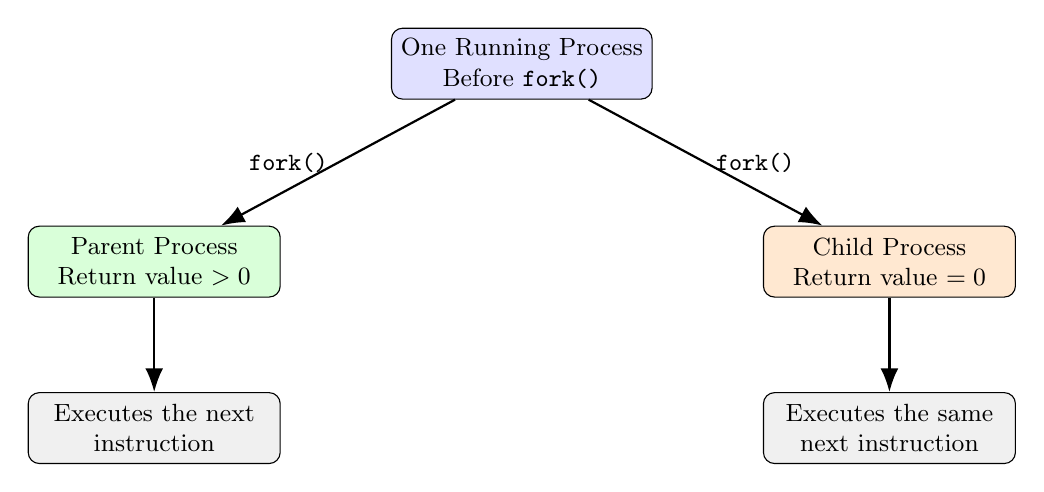
\begin{tikzpicture}[
    node distance=1.6cm,
    process/.style={
        draw,
        rounded corners,
        minimum width=3.2cm,
        minimum height=0.9cm,
        align=center,
        font=\small
    }
]

\node[process, fill=blue!12] (before)
{One Running Process\\Before \texttt{fork()}};

\node[process, fill=green!15,
below left=1.6cm and 1.4cm of before] (parent)
{Parent Process\\Return value $>0$};

\node[process, fill=orange!18,
below right=1.6cm and 1.4cm of before] (child)
{Child Process\\Return value $=0$};

\node[process, fill=gray!12,
below=1.2cm of parent] (parentnext)
{Executes the next\\instruction};

\node[process, fill=gray!12,
below=1.2cm of child] (childnext)
{Executes the same\\next instruction};

\draw[-{Latex[length=3mm]}, thick]
(before) -- node[left, font=\small]{\texttt{fork()}} (parent);

\draw[-{Latex[length=3mm]}, thick]
(before) -- node[right, font=\small]{\texttt{fork()}} (child);

\draw[-{Latex[length=3mm]}, thick]
(parent) -- (parentnext);

\draw[-{Latex[length=3mm]}, thick]
(child) -- (childnext);

\end{tikzpicture}
\end{center}

\end{frame}

% =====================================================
% SLIDE 9
% =====================================================
\begin{frame}{Parent and Child after \texttt{fork()}}

The child inherits copies of several properties from the parent.

\begin{itemize}
    \item Program code and execution context
    \item Environment variables
    \item Open file descriptors
    \item Current working directory
    \item User and group credentials
    \item Signal dispositions
\end{itemize}

However, parent and child differ in important ways:

\begin{itemize}
    \item They have different process IDs.
    \item The child has a different parent process ID.
    \item They have separate virtual address spaces.
    \item Changes made by one process to ordinary variables do not directly
    modify the other process's variables.
    \item The return value of \texttt{fork()} is different in each process.
\end{itemize}

\end{frame}

% =====================================================
% SLIDE 10
% =====================================================
\begin{frame}{Copy-on-Write}

\begin{block}{Concept}
Modern operating systems generally implement \texttt{fork()} using
\textbf{Copy-on-Write}, abbreviated as CoW.
\end{block}

\begin{itemize}
    \item The operating system does not immediately copy every memory page.
    \item Parent and child initially refer to the same physical memory pages.
    \item Shared pages are marked so that they cannot be modified directly.
    \item When either process modifies a page, the operating system creates a
    private copy of that page.
    \item This makes process creation faster and more memory-efficient.
\end{itemize}

\begin{alertblock}{Important}
Parent and child have logically separate address spaces even when physical pages
are temporarily shared through Copy-on-Write.
\end{alertblock}

\end{frame}

% =====================================================
% SLIDE 11
% =====================================================
\begin{frame}{The \texttt{getpid()} System Call}

\begin{block}{Purpose}
\texttt{getpid()} returns the Process ID of the calling process.
\end{block}

\begin{block}{Prototype}
\centering
\texttt{pid\_t getpid(void);}
\end{block}

\begin{itemize}
    \item It requires the header file \texttt{<unistd.h>}.
    \item It takes no arguments.
    \item It does not create a process.
    \item It identifies the process that is currently executing the statement.
    \item After \texttt{fork()}, parent and child obtain different values from
    \texttt{getpid()}.
\end{itemize}

\begin{exampleblock}{Example}
\centering
\texttt{printf("Current PID = \%d", (int)getpid());}
\end{exampleblock}

\end{frame}

% =====================================================
% SLIDE 12
% =====================================================
\begin{frame}{The \texttt{getppid()} System Call}

\begin{block}{Purpose}
\texttt{getppid()} returns the Process ID of the parent of the calling process.
\end{block}

\begin{block}{Prototype}
\centering
\texttt{pid\_t getppid(void);}
\end{block}

\begin{itemize}
    \item It requires the header file \texttt{<unistd.h>}.
    \item It takes no arguments.
    \item A child can identify its immediate parent using \texttt{getppid()}.
    \item If the original parent terminates, the child's parent may change after
    re-parenting by the operating system.
\end{itemize}

\begin{exampleblock}{Example}
\centering
\texttt{printf("Parent PID = \%d", (int)getppid());}
\end{exampleblock}

\end{frame}

% =====================================================
% SLIDE 13
% =====================================================
\begin{frame}[fragile]{Program: Identifying Parent and Child}

\begin{lstlisting}[style=cstyle]
#include <stdio.h>
#include <stdlib.h>
#include <unistd.h>

int main(void)
{
    pid_t pid = fork();

    if (pid < 0)
    {
        perror("fork failed");
        return EXIT_FAILURE;
    }
    else if (pid == 0)
    {
        printf("Child process\n");
        printf("Child PID  = %d\n", (int)getpid());
        printf("Parent PID = %d\n", (int)getppid());
    }
    else
    {
        printf("Parent process\n");
        printf("Parent PID = %d\n", (int)getpid());
        printf("Child PID  = %d\n", (int)pid);
    }

    return EXIT_SUCCESS;
}
\end{lstlisting}

\end{frame}

% =====================================================
% SLIDE 14
% =====================================================
\begin{frame}{Explanation of the Identification Program}

\begin{itemize}
    \item \texttt{pid = fork()} creates a child process.
    \item If \texttt{pid < 0}, process creation failed.
    \item If \texttt{pid == 0}, the code is executing in the child.
    \item If \texttt{pid > 0}, the code is executing in the parent.
    \item In the parent, \texttt{pid} contains the child's process ID.
    \item In the child, \texttt{getpid()} returns the child's own PID.
    \item In the child, \texttt{getppid()} returns the parent's PID.
\end{itemize}

\begin{alertblock}{Output Ordering}
The child may print before the parent, or the parent may print before the child.
The order is controlled by the scheduler unless explicit synchronization is used.
\end{alertblock}

\end{frame}

% =====================================================
% SLIDE 15
% =====================================================
\begin{frame}[fragile]{Program 1: Single \texttt{fork()}}

\begin{lstlisting}[style=cstyle]
#include <stdio.h>
#include <stdlib.h>
#include <unistd.h>

int main(void)
{
    pid_t pid = fork();

    if (pid < 0)
    {
        perror("fork failed");
        return EXIT_FAILURE;
    }

    printf("LINUX\n");

    return EXIT_SUCCESS;
}
\end{lstlisting}

\begin{block}{Observation}
The statement \texttt{printf("LINUX\textbackslash n");} is executed by both the
parent and the child.
\end{block}

\end{frame}

% =====================================================
% SLIDE 16
% =====================================================
\begin{frame}{Program 1: Expected Result}

\begin{columns}

\column{0.42\textwidth}

\begin{block}{Possible Output}
\texttt{LINUX}\\
\texttt{LINUX}
\end{block}

\column{0.54\textwidth}

\begin{itemize}
    \item Initially, one process exists.
    \item One \texttt{fork()} creates one child.
    \item Total processes after \texttt{fork()} are two.
    \item Both processes execute the next statement.
    \item Therefore, the message is printed twice.
\end{itemize}

\end{columns}

\vspace{0.4cm}

\begin{center}
\Large
\[
\text{Total processes}=2^1=2
\]
\end{center}

\end{frame}

% =====================================================
% SLIDE 17
% =====================================================
\begin{frame}{Output Buffering and \texttt{fork()}}

Standard output may be buffered.

\begin{itemize}
    \item A newline usually flushes a terminal line buffer.
    \item Output without a newline may remain in the user-space buffer.
    \item When \texttt{fork()} is called, the child receives a copy of the
    process's output buffer.
    \item Both processes may later flush the copied buffer.
    \item This may cause text written before \texttt{fork()} to appear more than
    once.
\end{itemize}

\begin{alertblock}{Good Practice}
Use a newline or call \texttt{fflush(stdout)} before \texttt{fork()} when output
buffering may affect the experiment.
\end{alertblock}

\end{frame}

% =====================================================
% SLIDE 18
% =====================================================
\begin{frame}[fragile]{Buffering Example}

\begin{lstlisting}[style=cstyle]
#include <stdio.h>
#include <unistd.h>

int main(void)
{
    printf("Before fork");

    fork();

    printf(" After fork\n");

    return 0;
}
\end{lstlisting}

\begin{block}{Observation}
When output is redirected to a file, the text \texttt{Before fork} may be copied
with the output buffer and printed by both processes.
\end{block}

\begin{exampleblock}{Safer Version}
Use \texttt{printf("Before fork\textbackslash n");} or call
\texttt{fflush(stdout);} before \texttt{fork()}.
\end{exampleblock}

\end{frame}

% =====================================================
% SLIDE 19
% =====================================================
\begin{frame}{What is \texttt{wait()}?}

\begin{block}{Definition}
\texttt{wait()} suspends the calling parent process until one of its child
processes terminates or changes state.
\end{block}

\begin{block}{Header and Prototype}
\centering
\texttt{\#include <sys/wait.h>}\\[0.15cm]
\texttt{pid\_t wait(int *status);}
\end{block}

\begin{itemize}
    \item It is normally called by a parent process.
    \item It returns the PID of the child whose status was collected.
    \item It can collect the child's termination status.
    \item It helps prevent terminated children from remaining as zombies.
    \item \texttt{wait(NULL)} may be used when the exit status is not required.
\end{itemize}

\end{frame}

% =====================================================
% SLIDE 20
% =====================================================
\begin{frame}[fragile]{Program: Parent Waits for Child}

\begin{lstlisting}[style=cstyle]
#include <stdio.h>
#include <stdlib.h>
#include <unistd.h>
#include <sys/wait.h>

int main(void)
{
    pid_t pid = fork();

    if (pid < 0)
    {
        perror("fork failed");
        return EXIT_FAILURE;
    }
    else if (pid == 0)
    {
        printf("Child is executing\n");
        printf("Child PID = %d\n", (int)getpid());
        sleep(2);
        printf("Child has completed\n");
        exit(EXIT_SUCCESS);
    }
    else
    {
        wait(NULL);
        printf("Parent resumes after child completion\n");
    }

    return EXIT_SUCCESS;
}
\end{lstlisting}

\end{frame}

% =====================================================
% SLIDE 21
% =====================================================
\begin{frame}{Working of \texttt{wait()}}

\begin{enumerate}
    \item The parent creates a child using \texttt{fork()}.
    \item The child executes its assigned statements.
    \item The parent calls \texttt{wait(NULL)}.
    \item If the child is still running, the parent becomes blocked.
    \item When the child terminates, the operating system records its status.
    \item \texttt{wait()} collects the child status.
    \item The parent becomes ready to execute again.
\end{enumerate}

\begin{alertblock}{Scheduling vs Synchronization}
Without \texttt{wait()}, output order depends on scheduling. With
\texttt{wait()}, statements after \texttt{wait()} execute only after a child has
terminated.
\end{alertblock}

\end{frame}

% =====================================================
% SLIDE 22
% =====================================================
\begin{frame}{Collecting the Child's Exit Status}

The parent can inspect the child's termination information using macros from
\texttt{<sys/wait.h>}.

\begin{itemize}
    \item \texttt{WIFEXITED(status)} checks whether the child terminated normally.
    \item \texttt{WEXITSTATUS(status)} obtains the child's exit status.
    \item \texttt{WIFSIGNALED(status)} checks whether a signal terminated the
    child.
    \item \texttt{WTERMSIG(status)} obtains the terminating signal number.
    \item \texttt{WIFSTOPPED(status)} checks whether the child was stopped.
\end{itemize}

\begin{alertblock}{Restriction}
Use \texttt{WEXITSTATUS(status)} only when
\texttt{WIFEXITED(status)} evaluates to true.
\end{alertblock}

\end{frame}

% =====================================================
% SLIDE 23
% =====================================================
\begin{frame}[fragile]{Program: Reading Exit Status}

\begin{lstlisting}[style=cstyle]
#include <stdio.h>
#include <stdlib.h>
#include <unistd.h>
#include <sys/wait.h>

int main(void)
{
    pid_t pid = fork();
    int status;

    if (pid < 0)
    {
        perror("fork failed");
        return EXIT_FAILURE;
    }
    else if (pid == 0)
    {
        printf("Child is exiting with status 7\n");
        exit(7);
    }
    else
    {
        wait(&status);

        if (WIFEXITED(status))
        {
            printf("Child exit status = %d\n",
                   WEXITSTATUS(status));
        }
    }

    return EXIT_SUCCESS;
}
\end{lstlisting}

\end{frame}

% =====================================================
% SLIDE 24
% =====================================================
\begin{frame}{What is \texttt{waitpid()}?}

\begin{block}{Prototype}
\centering
\texttt{pid\_t waitpid(pid\_t pid, int *status, int options);}
\end{block}

\begin{itemize}
    \item \texttt{waitpid()} provides more control than \texttt{wait()}.
    \item It can wait for a specific child process.
    \item It can perform non-blocking status checks using \texttt{WNOHANG}.
    \item With \texttt{pid > 0}, it waits for the child having that PID.
    \item With \texttt{pid = -1}, it behaves similarly to \texttt{wait()}.
\end{itemize}

\begin{exampleblock}{Example}
\centering
\texttt{waitpid(child\_pid, \&status, 0);}
\end{exampleblock}

\end{frame}

% =====================================================
% SLIDE 25
% =====================================================
\begin{frame}{Process Termination: \texttt{return}, \texttt{exit()} and \texttt{\_exit()}}

\begin{description}
    \item[\texttt{return} from \texttt{main}:]
    Terminates the process and provides an exit status.

    \item[\texttt{exit(status)}:]
    Performs normal process termination, flushes standard I/O buffers and invokes
    registered exit handlers.

    \item[\texttt{\_exit(status)}:]
    Terminates immediately without normal standard-I/O cleanup.
\end{description}

\begin{alertblock}{After \texttt{fork()}}
In a child that fails to execute a new program after an \texttt{exec()} call,
\texttt{\_exit()} is often preferred to avoid flushing copied parent-side I/O
buffers.
\end{alertblock}

\end{frame}

% =====================================================
% SLIDE 26
% =====================================================
\begin{frame}{Zombie Process}

\begin{block}{Definition}
A zombie is a child process that has terminated, but whose termination status has
not yet been collected by its parent.
\end{block}

\begin{itemize}
    \item The child has completed execution.
    \item Most of its resources have been released.
    \item A small process-table entry is retained.
    \item The entry stores termination information needed by the parent.
    \item The parent removes the zombie by calling \texttt{wait()} or
    \texttt{waitpid()}.
\end{itemize}

\begin{alertblock}{Important}
A zombie does not continue executing, but excessive unreaped zombies can consume
process-table entries.
\end{alertblock}

\end{frame}

% =====================================================
% SLIDE 27
% =====================================================
\begin{frame}[fragile]{Program: Demonstrating a Zombie Process}

\begin{lstlisting}[style=cstyle]
#include <stdio.h>
#include <stdlib.h>
#include <unistd.h>

int main(void)
{
    pid_t pid = fork();

    if (pid < 0)
    {
        perror("fork failed");
        return EXIT_FAILURE;
    }
    else if (pid == 0)
    {
        printf("Child is terminating\n");
        exit(EXIT_SUCCESS);
    }
    else
    {
        printf("Parent is sleeping without wait()\n");
        sleep(20);
    }

    return EXIT_SUCCESS;
}
\end{lstlisting}

\begin{block}{Observation Command}
During the parent's sleep, inspect processes using:
\texttt{ps -el | grep Z}
\end{block}

\end{frame}

% =====================================================
% SLIDE 28
% =====================================================
\begin{frame}{Orphan Process}

\begin{block}{Definition}
An orphan is a running child process whose original parent terminates before the
child.
\end{block}

\begin{itemize}
    \item The child does not necessarily terminate when its parent exits.
    \item The operating system re-parents the orphan.
    \item A system process or subreaper may become its new parent.
    \item The value returned by \texttt{getppid()} may therefore change.
\end{itemize}

\begin{alertblock}{Comparison}
A zombie has already terminated but has not been reaped. An orphan is still
running after its original parent terminates.
\end{alertblock}

\end{frame}

% =====================================================
% SLIDE 29
% =====================================================
\begin{frame}[fragile]{Program: Demonstrating an Orphan Process}

\begin{lstlisting}[style=cstyle]
#include <stdio.h>
#include <stdlib.h>
#include <unistd.h>

int main(void)
{
    pid_t pid = fork();

    if (pid < 0)
    {
        perror("fork failed");
        return EXIT_FAILURE;
    }
    else if (pid == 0)
    {
        printf("Original parent PID = %d\n",
               (int)getppid());

        sleep(5);

        printf("New parent PID = %d\n",
               (int)getppid());
    }
    else
    {
        printf("Parent is terminating\n");
        exit(EXIT_SUCCESS);
    }

    return EXIT_SUCCESS;
}
\end{lstlisting}

\end{frame}

% =====================================================
% SLIDE 30
% =====================================================
\begin{frame}{The \texttt{exec()} Family}

\begin{block}{Purpose}
The \texttt{exec()} family replaces the current process image with a new program.
\end{block}

\begin{itemize}
    \item \texttt{exec()} does not create an additional process.
    \item The calling process keeps its PID.
    \item Its code, data, stack, and heap are replaced by the new program.
    \item On success, an \texttt{exec()} function does not return.
    \item On failure, it returns \texttt{-1} and sets \texttt{errno}.
\end{itemize}

Common functions include:

\begin{center}
\texttt{execl()}, \texttt{execlp()}, \texttt{execle()},
\texttt{execv()}, \texttt{execvp()}, and \texttt{execve()}
\end{center}

\end{frame}

% =====================================================
% SLIDE 31
% =====================================================
\begin{frame}[fragile]{Program: \texttt{fork()} with \texttt{exec()}}

\begin{lstlisting}[style=cstyle]
#include <stdio.h>
#include <stdlib.h>
#include <unistd.h>
#include <sys/wait.h>

int main(void)
{
    pid_t pid = fork();

    if (pid < 0)
    {
        perror("fork failed");
        return EXIT_FAILURE;
    }
    else if (pid == 0)
    {
        execlp("ls", "ls", "-l", NULL);

        perror("execlp failed");
        _exit(EXIT_FAILURE);
    }
    else
    {
        wait(NULL);
        printf("Parent: command completed\n");
    }

    return EXIT_SUCCESS;
}
\end{lstlisting}

\end{frame}

% =====================================================
% SLIDE 32
% =====================================================
\begin{frame}{Standard \texttt{fork()}--\texttt{exec()}--\texttt{wait()} Pattern}

\begin{center}
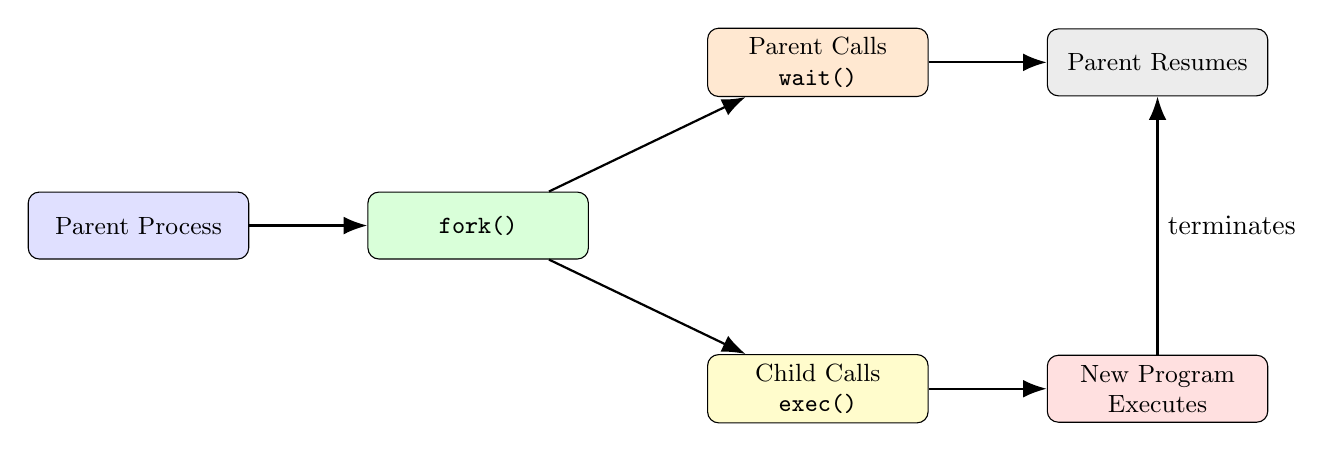
\begin{tikzpicture}[
    node distance=1.5cm,
    box/.style={
        draw,
        rounded corners,
        minimum width=2.8cm,
        minimum height=0.85cm,
        align=center,
        font=\small
    }
]

\node[box, fill=blue!12] (parent)
{Parent Process};

\node[box, fill=green!15, right=1.5cm of parent] (fork)
{\texttt{fork()}};

\node[box, fill=orange!18,
above right=1.2cm and 1.5cm of fork] (parentwait)
{Parent Calls\\\texttt{wait()}};

\node[box, fill=yellow!20,
below right=1.2cm and 1.5cm of fork] (childexec)
{Child Calls\\\texttt{exec()}};

\node[box, fill=red!12,
right=1.5cm of childexec] (program)
{New Program\\Executes};

\node[box, fill=gray!15,
right=1.5cm of parentwait] (resume)
{Parent Resumes};

\draw[-{Latex[length=3mm]}, thick] (parent) -- (fork);
\draw[-{Latex[length=3mm]}, thick] (fork) -- (parentwait);
\draw[-{Latex[length=3mm]}, thick] (fork) -- (childexec);
\draw[-{Latex[length=3mm]}, thick] (childexec) -- (program);
\draw[-{Latex[length=3mm]}, thick] (program) -- node[right]{terminates} (resume);
\draw[-{Latex[length=3mm]}, thick] (parentwait) -- (resume);

\end{tikzpicture}
\end{center}

\end{frame}

% =====================================================
% SLIDE 33
% =====================================================
\begin{frame}{Comparison of Related Process Functions}

\begin{center}
\small
\begin{tabular}{|p{2.2cm}|p{8.8cm}|}
\hline
\textbf{Function} & \textbf{Purpose} \\
\hline
\texttt{fork()} &
Creates a new child process by duplicating the caller. \\
\hline
\texttt{getpid()} &
Returns the PID of the calling process. \\
\hline
\texttt{getppid()} &
Returns the PID of the calling process's parent. \\
\hline
\texttt{wait()} &
Waits for any eligible child and collects its status. \\
\hline
\texttt{waitpid()} &
Waits for a selected child or performs controlled status checking. \\
\hline
\texttt{exec()} &
Replaces the current process image with a new program. \\
\hline
\texttt{exit()} &
Performs normal process termination. \\
\hline
\texttt{\_exit()} &
Terminates immediately without normal standard-I/O cleanup. \\
\hline
\end{tabular}
\end{center}

\end{frame}

% =====================================================
% SLIDE 34
% =====================================================
\begin{frame}[fragile]{Program 2: Multiple \texttt{fork()} Calls}

\begin{lstlisting}[style=cstyle]
#include <stdio.h>
#include <stdlib.h>
#include <unistd.h>

int main(void)
{
    fork();
    printf("LINUX\n");

    fork();
    printf("UNIX\n");

    fork();
    printf("RED HAT\n");

    return EXIT_SUCCESS;
}
\end{lstlisting}

\begin{alertblock}{Assumption}
This example focuses on successful process creation. In production-quality code,
the return value of every \texttt{fork()} call should be checked.
\end{alertblock}

\end{frame}

% =====================================================
% SLIDE 35
% =====================================================
\begin{frame}{Process Growth after Multiple \texttt{fork()} Calls}

\begin{center}
\begin{tabular}{|c|c|c|}
\hline
\textbf{Execution Stage} &
\textbf{Running Processes} &
\textbf{New Output Count} \\
\hline
Before any \texttt{fork()} & 1 & 0 \\
\hline
After first \texttt{fork()} & 2 & LINUX: 2 times \\
\hline
After second \texttt{fork()} & 4 & UNIX: 4 times \\
\hline
After third \texttt{fork()} & 8 & RED HAT: 8 times \\
\hline
\end{tabular}
\end{center}

\vspace{0.4cm}

\begin{block}{Formula}
For \(n\) successive independent \texttt{fork()} calls executed by every existing
process:
\[
\text{Total processes}=2^n
\]
\[
\text{New child processes}=2^n-1
\]
\end{block}

\end{frame}

% =====================================================
% SLIDE 36
% =====================================================
\begin{frame}{Process Tree for Three Successive \texttt{fork()} Calls}

\begin{center}
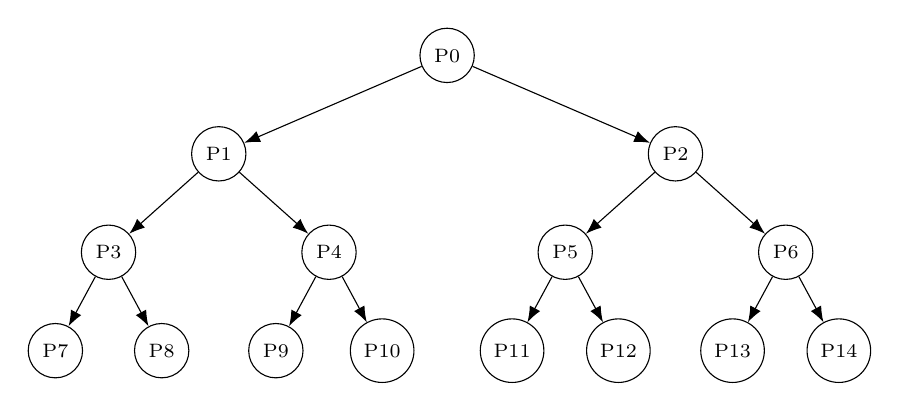
\begin{tikzpicture}[
    level 1/.style={sibling distance=5.8cm, level distance=1.25cm},
    level 2/.style={sibling distance=2.8cm, level distance=1.25cm},
    level 3/.style={sibling distance=1.35cm, level distance=1.25cm},
    every node/.style={
        draw,
        circle,
        minimum size=0.65cm,
        font=\scriptsize
    },
    edge from parent/.style={
        draw,
        -{Latex[length=2mm]}
    }
]

\node {P0}
child {node {P1}
    child {node {P3}
        child {node {P7}}
        child {node {P8}}
    }
    child {node {P4}
        child {node {P9}}
        child {node {P10}}
    }
}
child {node {P2}
    child {node {P5}
        child {node {P11}}
        child {node {P12}}
    }
    child {node {P6}
        child {node {P13}}
        child {node {P14}}
    }
};

\end{tikzpicture}
\end{center}

\begin{alertblock}{Conceptual Representation}
Each level represents another \texttt{fork()} executed by every process existing
at that point. Process identifiers shown here are logical labels, not actual
system-assigned PIDs.
\end{alertblock}

\end{frame}

% =====================================================
% SLIDE 37
% =====================================================
\begin{frame}{Possible Output of the Multiple-Fork Program}

\begin{columns}

\column{0.44\textwidth}

\begin{block}{Output Counts}
\begin{itemize}
    \item LINUX: 2 times
    \item UNIX: 4 times
    \item RED HAT: 8 times
\end{itemize}
\end{block}

\column{0.52\textwidth}

\begin{block}{Total Printed Lines}
\[
2+4+8=14
\]
\end{block}

\begin{itemize}
    \item Exact line order may vary.
    \item Scheduling differs across runs.
    \item Output count remains predictable when all calls succeed.
\end{itemize}

\end{columns}

\end{frame}

% =====================================================
% SLIDE 38
% =====================================================
\begin{frame}{Common Errors and Precautions}

\begin{itemize}
    \item Compiling \texttt{fork()} code with a native Windows compiler.
    \item Forgetting to include \texttt{<unistd.h>}.
    \item Forgetting to include \texttt{<sys/wait.h>} for \texttt{wait()}.
    \item Ignoring a negative return value from \texttt{fork()}.
    \item Assuming the parent always executes before the child.
    \item Creating an uncontrolled number of processes.
    \item Forgetting to reap terminated children.
    \item Using output statements before \texttt{fork()} without considering
    buffering.
\end{itemize}

\begin{alertblock}{Warning}
Avoid running fork-intensive programs without calculating the number of processes
first. Uncontrolled process creation can exhaust system resources.
\end{alertblock}

\end{frame}

% =====================================================
% SLIDE 39
% =====================================================
\begin{frame}{Linux Lab Execution Steps}

\begin{enumerate}
    \item Open a Linux or Ubuntu terminal.
    \item Create the source file:
    \begin{center}
        \texttt{nano forkdemo.c}
    \end{center}
    \item Enter the C program and save the file.
    \item Compile with warnings enabled:
    \begin{center}
        \texttt{gcc -Wall -Wextra forkdemo.c -o forkdemo}
    \end{center}
    \item Execute the program:
    \begin{center}
        \texttt{./forkdemo}
    \end{center}
    \item Run the program several times and compare output ordering.
    \item View process information using \texttt{ps}, \texttt{pstree}, or
    \texttt{top}.
\end{enumerate}

\end{frame}

% =====================================================
% SLIDE 40
% =====================================================
\begin{frame}{Useful Linux Commands}

\begin{center}
\begin{tabular}{|p{3.2cm}|p{7.8cm}|}
\hline
\textbf{Command} & \textbf{Purpose} \\
\hline
\texttt{ps} & Displays processes associated with the current terminal. \\
\hline
\texttt{ps -ef} & Displays detailed information about running processes. \\
\hline
\texttt{pstree -p} & Displays process hierarchy along with PIDs. \\
\hline
\texttt{top} & Displays dynamically updated process information. \\
\hline
\texttt{man 2 fork} & Opens the manual page for the \texttt{fork()} system call. \\
\hline
\texttt{man 2 wait} & Opens the manual page for process waiting functions. \\
\hline
\texttt{kill PID} & Sends a termination signal to a selected process. \\
\hline
\end{tabular}
\end{center}

\end{frame}

% =====================================================
% SLIDE 41
% =====================================================
\begin{frame}{Classwork}

\begin{enumerate}
    \item Write a program that creates one child and prints the PID and PPID of
    both parent and child.

    \item Use the return value of \texttt{fork()} to print ``Parent Process'' only
    in the parent and ``Child Process'' only in the child.

    \item Write a program in which the child prints numbers from 1 to 5 and the
    parent waits for it using \texttt{wait()}.

    \item Execute two successive \texttt{fork()} calls. Predict the number of
    processes and draw the process tree.

    \item Modify the single-\texttt{fork()} program to print the value returned by
    \texttt{fork()} in both processes.
\end{enumerate}

\end{frame}

% =====================================================
% SLIDE 42
% =====================================================
\begin{frame}{Homework}

\begin{enumerate}
    \item Write a program in which the parent prints even numbers from 1 to 20
    and the child prints odd numbers.

    \item Create three child processes. Each child must print its PID, PPID, and
    child number.

    \item Write a program where the child exits with status 10 and the parent
    reads the status using \texttt{wait()}.

    \item Demonstrate an orphan process and record the child's PPID before and
    after the parent terminates.

    \item Demonstrate a zombie process and observe it using the \texttt{ps}
    command.

    \item Write a program using \texttt{fork()}, \texttt{exec()}, and
    \texttt{wait()} to execute the \texttt{date} command.
\end{enumerate}

\end{frame}

% =====================================================
% SLIDE 43
% =====================================================
\begin{frame}{Viva Questions}

\begin{enumerate}
    \item Why is \texttt{fork()} described as being called once but returning
    twice?
    \item What values does \texttt{fork()} return in the parent and child?
    \item What is the difference between \texttt{getpid()} and
    \texttt{getppid()}?
    \item Why is \texttt{wait()} required?
    \item What is the difference between an orphan and a zombie?
    \item Does \texttt{exec()} create a new process?
    \item What is Copy-on-Write?
    \item Why can output order vary after \texttt{fork()}?
    \item How many processes exist after four successive independent
    \texttt{fork()} calls?
    \item What happens when \texttt{fork()} fails?
\end{enumerate}

\end{frame}

% =====================================================
% SLIDE 44
% =====================================================
\begin{frame}{Summary}

\begin{itemize}
    \item \texttt{fork()} creates a new child process.
    \item Parent and child continue from the next instruction.
    \item The child receives 0 and the parent receives the child's PID.
    \item \texttt{getpid()} identifies the current process.
    \item \texttt{getppid()} identifies the parent process.
    \item \texttt{wait()} synchronizes the parent with child termination.
    \item \texttt{exec()} replaces the current process image.
    \item Unreaped terminated children become zombies.
    \item Running children whose parents terminate become orphans.
    \item Multiple successive \texttt{fork()} calls may increase the number of
    processes exponentially.
\end{itemize}

\begin{center}
\vspace{0.3cm}
\Large\textbf{Week 1 Operating Systems Lab Completed}
\end{center}

\end{frame}

% =====================================================
% SLIDE 45
% =====================================================
\begin{frame}{References}

\small

\begin{thebibliography}{9}

\bibitem{osc}
Abraham Silberschatz, Peter B. Galvin, and Greg Gagne,
\newblock \emph{Operating System Concepts},
\newblock Wiley.

\bibitem{mos}
Andrew S. Tanenbaum and Herbert Bos,
\newblock \emph{Modern Operating Systems},
\newblock Pearson.

\bibitem{apue}
W. Richard Stevens and Stephen A. Rago,
\newblock \emph{Advanced Programming in the UNIX Environment},
\newblock Addison-Wesley.

\bibitem{linux}
Michael Kerrisk,
\newblock \emph{The Linux Programming Interface},
\newblock No Starch Press.

\bibitem{manual}
Linux Programmer's Manual,
\newblock \texttt{fork(2)}, \texttt{getpid(2)}, \texttt{wait(2)},
\texttt{execve(2)}, and \texttt{exit(3)}.

\end{thebibliography}

\end{frame}

% =====================================================
% END
% =====================================================
\end{document}

